% =====================================================================
% fig:families_photos — compact FULL-WIDTH photo figure (figure*):
% single row: leftmost Source A, then one representative
% identity-matched MAD22 morph per family (FaceMorpher, OpenCV,
% WebMorph, MIPGAN-I, MIPGAN-II), rightmost Source B (010_03). All
% seven panels come from the same corrected corpus rows of one shared
% contributor pair (A = 001_03, B = 010_03); every morph in the row
% blends exactly these two contributors.
%
% Image source: native rows of the corrected MAD22 corpus
%   /mnt/t7/smad_heldout/mad22_canonical_E7_inputs_v3_20261109T113746Z
%   (sha256 of each panel preserved through downsampling in the
%   supplementary build manifest; volumes as in tab:mad22_results).
% REAL corpus imagery (unlike figures/teaser.tex and
% figures/families.tex). Two people per row, adults only.
% The FaceMorpher image retains its released generator watermark.
% Every panel is a genuinely retained row of the corrected
% benchmark; selection is descriptive only and part of no claim.
%
% Layout: no \resizebox, no node-nested inline \tikz (both are
% known hazards in this project); plain tabular + \includegraphics
% + \parbox labels. Smallest text: \tiny on \scriptsize panels.
% =====================================================================
\begin{figure*}[t]
\centering
\setlength{\tabcolsep}{2pt}%
\begin{tabular}{@{}c@{\hspace{3pt}}c@{\hspace{3pt}}c@{\hspace{3pt}}c@{\hspace{3pt}}c@{\hspace{3pt}}c@{\hspace{3pt}}c@{}}
  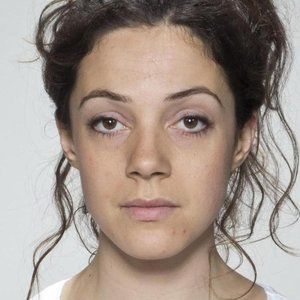
\includegraphics[width=0.125\textwidth]{families_photos/person001_photo.jpg} &
  \frame{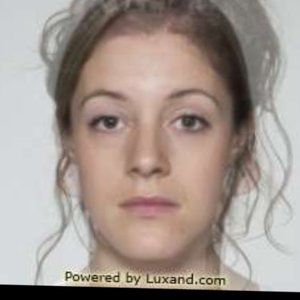
\includegraphics[width=0.125\textwidth]{families_photos/morph_facemorpher.jpg}} &
  \frame{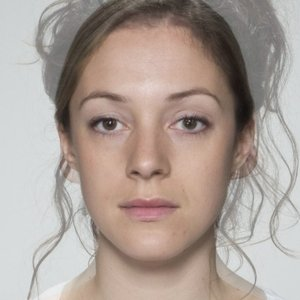
\includegraphics[width=0.125\textwidth]{families_photos/morph_opencv.jpg}} &
  \frame{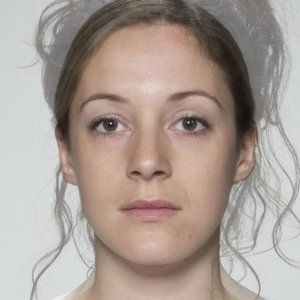
\includegraphics[width=0.125\textwidth]{families_photos/morph_webmorph.jpg}} &
  \frame{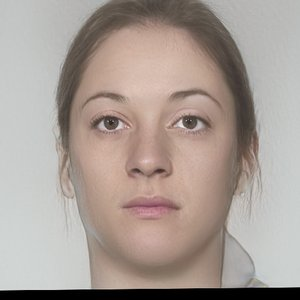
\includegraphics[width=0.125\textwidth]{families_photos/morph_mipgan1.jpg}} &
  \frame{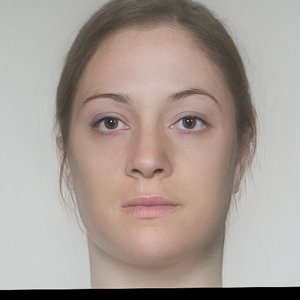
\includegraphics[width=0.125\textwidth]{families_photos/morph_mipgan2.jpg}} &
  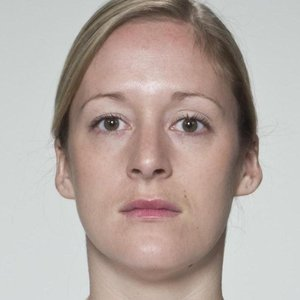
\includegraphics[width=0.125\textwidth]{families_photos/person010_photo.jpg}\\[3pt]
  {\tiny\sffamily\textbf{Source A}} &
  {\tiny\sffamily\textbf{FaceMorpher}} &
  {\tiny\sffamily\textbf{OpenCV}} &
  {\tiny\sffamily\textbf{WebMorph}} &
  {\tiny\sffamily\textbf{MIPGAN-I}} &
  {\tiny\sffamily\textbf{MIPGAN-II}} &
  {\tiny\sffamily\textbf{Source B}}\\[-1pt]
  {\tiny\sffamily contributor 001\_03} &
  \parbox[t]{0.135\textwidth}{\centering\tiny\sffamily halo ring + sharpness/energy} &
  \parbox[t]{0.135\textwidth}{\centering\tiny\sffamily halo + warp-only surround} &
  \parbox[t]{0.135\textwidth}{\centering\tiny\sffamily halo ring + illumination/pose} &
  \parbox[t]{0.135\textwidth}{\centering\tiny\sffamily GAN fingerprint response} &
  \parbox[t]{0.135\textwidth}{\centering\tiny\sffamily GAN fingerprint + sharpness} &
  {\tiny\sffamily contributor 010\_03}\\
\end{tabular}
\caption{Real examples of the five MAD22 morph families analyzed in
Sections~\ref{sec:matched_controls} and~\ref{sec:benchmark_results}. Every morph is a
genuine blend of the same two contributor photographs shown at the ends of
the row (A = 001\_03, B = 010\_03), drawn from the corrected benchmark;
the shortcut label under each panel names the non-identity trait our
instruments isolate for that family. Descriptive illustration only; not a
benchmark claim.}
\label{fig:families_photos}
\end{figure*}
